\begin{comment}
	\pagebreak
\end{comment}

\section{Recurrent Neural Network}
\begin{comment}
	The main advantage of RNN's over vanilla NN's or CNN's is the flexibility when it comes to input size.\\
	\textbf{NN} has a fixed input/output size and computes a fixed amount of computational steps (defined by number of layers).\\
	\textbf{RNN} can work over sequences of data, learning the transistion given the (implicitly stored) past data.\\
	
	\begin{Figure}
 		\centering
 		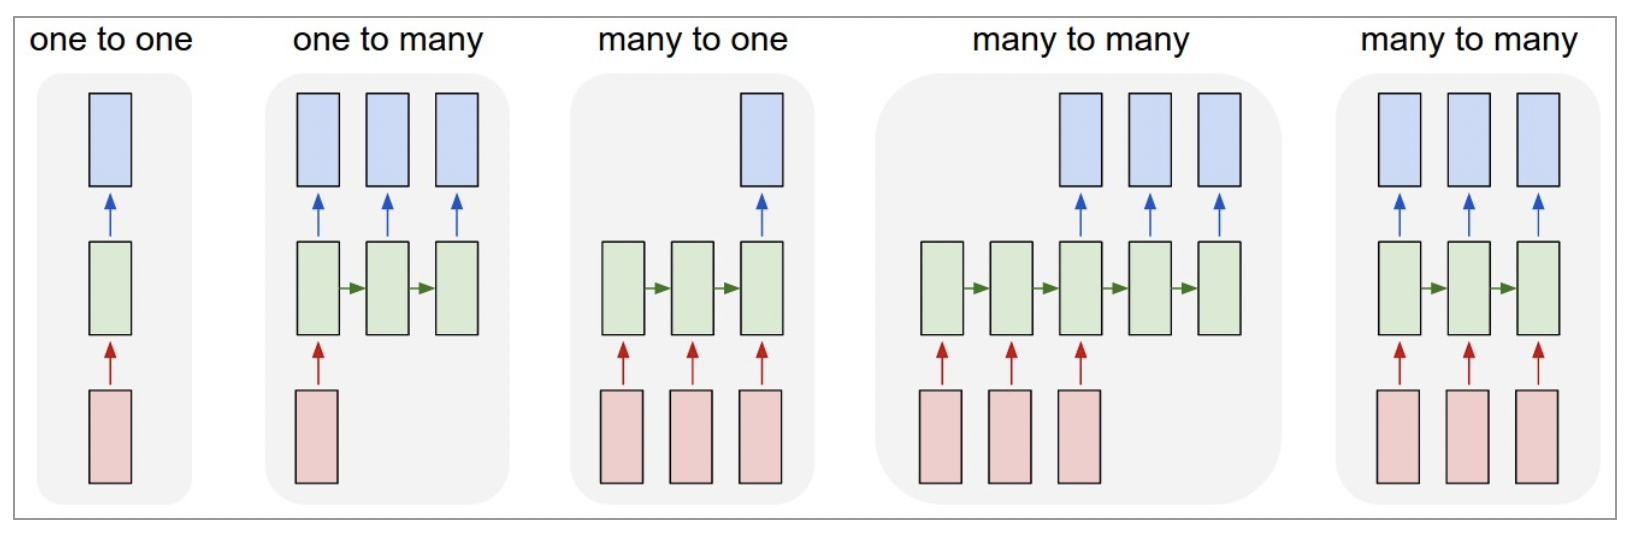
\includegraphics[width=\linewidth]{graphic/rnn-options}
 		\captionof{figure}{RNN 1. NN, 2. Image captioning, 3. Sentiment analysis, 4. Translation, 5. Video classification}
	\end{Figure} 
	\begin{Figure}
 		\centering
 		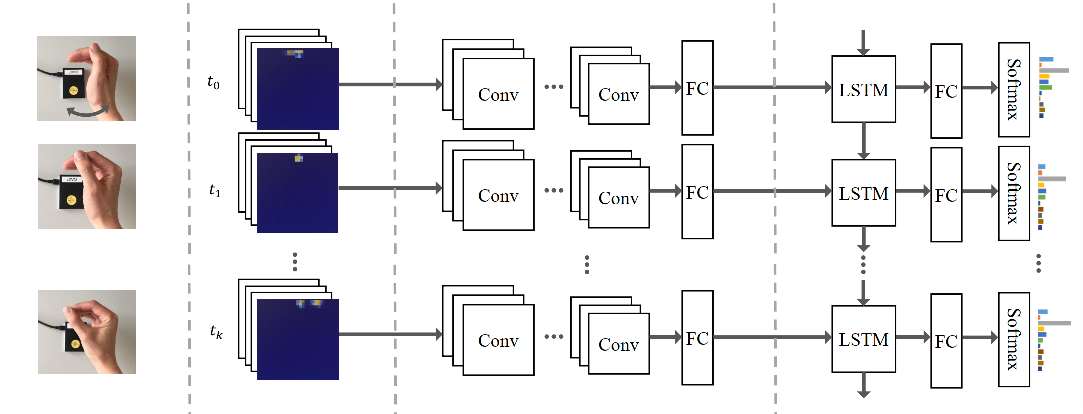
\includegraphics[width=\linewidth]{graphic/rnn-video-classification-architecture}
 		\captionof{figure}{RNN Video classification architecture}
	\end{Figure} 
\end{comment}

\textbf{Vanilla RNN:} $\why = W_{hy} h^t$, $h^t = tanh(W_{hh} h^{t-1} + W_{xh} x^t)$
\begin{comment}
	\textbf{Goal:} Learn transition function knowing what's worth keeping.
	Tanh is important, otherwise we can't forget information.\\

	\begin{Figure}
 		\centering
 		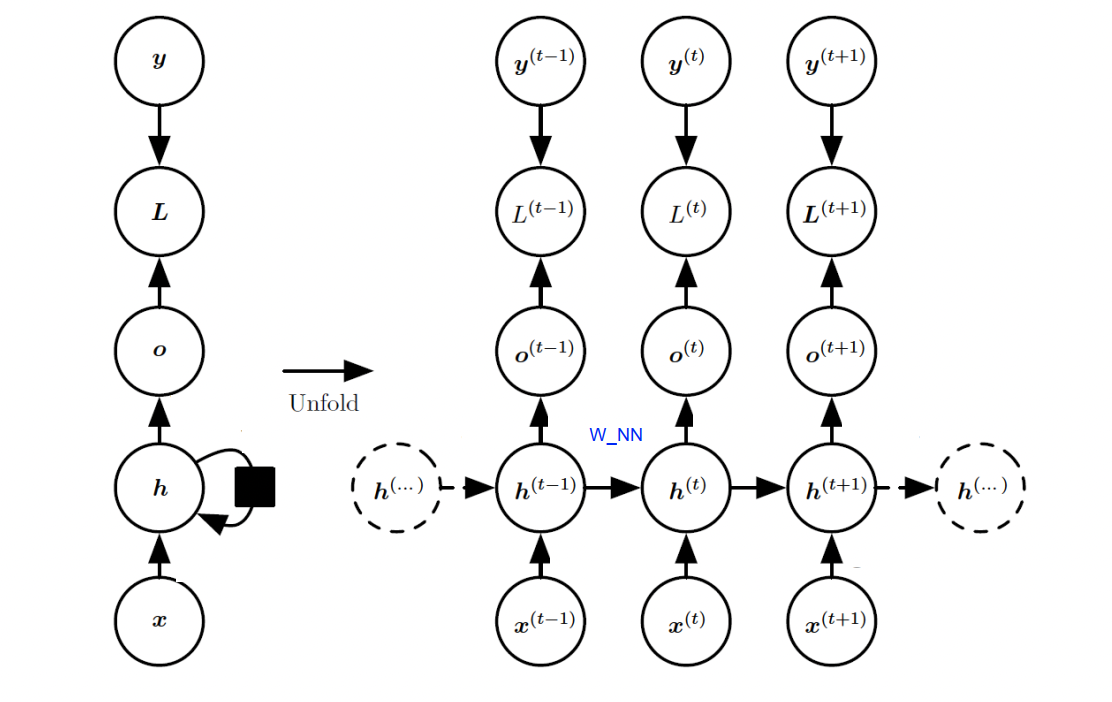
\includegraphics[width=\linewidth]{graphic/rnn-detailed}
 		\captionof{figure}{Visualisation of complex RNN}
	\end{Figure}
\end{comment}

\textbf{Backprop:} $\frac{\delta L}{\delta W} 
= \sum_{t=1}^S \frac{\delta L^t}{\delta W}
= \sum_{t=1}^S \sum_{k=1}^t \frac{\delta L^t}{\delta y^t} \frac{\delta y^t}{\delta h^t} \frac{\delta h^t}{\delta h^k} \frac{\delta^+ h^k}{\delta W}$\\
\todo{Understand this better}
\begin{comment}
	\begin{Figure}
 		\centering
 		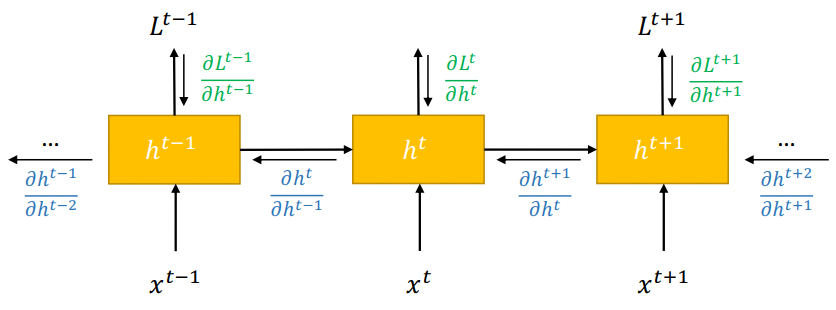
\includegraphics[width=\linewidth]{graphic/rnn-backprop-2}
 		\captionof{figure}{RNN Backprop unrolled}
	\end{Figure}
\end{comment}

\textbf{Gradient:} $h^t = W^T h^{t-1} = (W^T)^t h^1 = (Q^T \Lambda^t Q) h^1$\\
\begin{comment}
	The Eigenvalues of the weigh matrix explode or vanish when the sequence length gets to big.
	Regularizing the Eigenvalues is proven to reduce the learning capabilities of the learning-system drastically, and is thus not an option\\
	\textbf{Exploding gradients:} exploding gradients can be managed by clipping after a certain size\\
	\textbf{Vanishing gradients:} Add memory cell\\
	
	\begin{Figure}
 		\centering
 		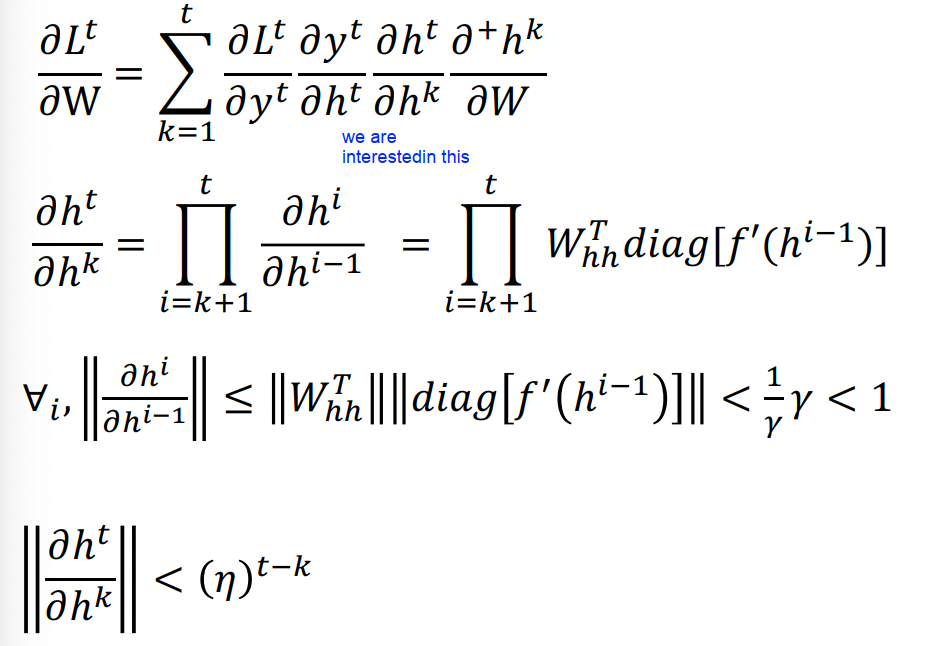
\includegraphics[width=\linewidth]{graphic/rnn-vanishing-gradient-proof}
 		\captionof{figure}{Proof that vanishing Gradients are a problem}
	\end{Figure}
\end{comment}

\textbf{LSTM:} $c_t^l = f \odot c_{t-1}^l + i \odot g$,
$h_t = o \odot tanh(c_t^l)$,\\
$f,i,o, g = [\sigma,\sigma,\sigma,tanh]\odot W^l[h_{t-1}^l h_t^{l-1}]^T$\\
\begin{comment}
	To mitigate the vanishing gradients, we introduce a long term memory unit. 
	There are three phases to this: forgetting, new information and output generation.\\
	1) Forgetting happens through manipulating $c$ with $f \in [0,1]$\\
	2) New information is compiled by trying to figure out what to add/ remove to the current memory, as $g \in [-1, 1]$\\
	3) Output generation is done by mixing the short-term input with the long-term memory\\

	\begin{Figure}
 		\centering
 		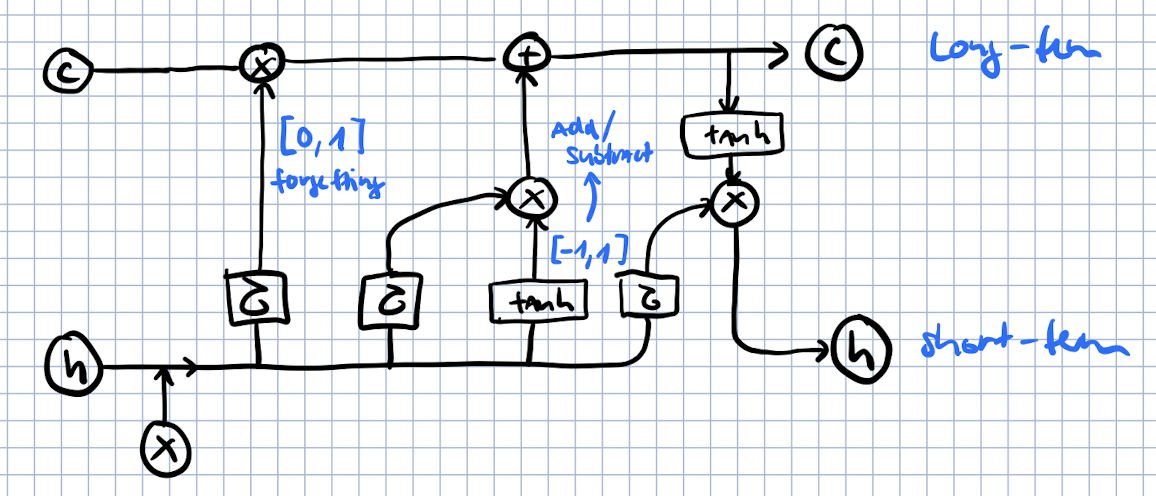
\includegraphics[width=\linewidth]{graphic/rnn-lstm-3}
 		\captionof{figure}{LSTM Visualization}
	\end{Figure}
		\begin{Figure}
 		\centering
 		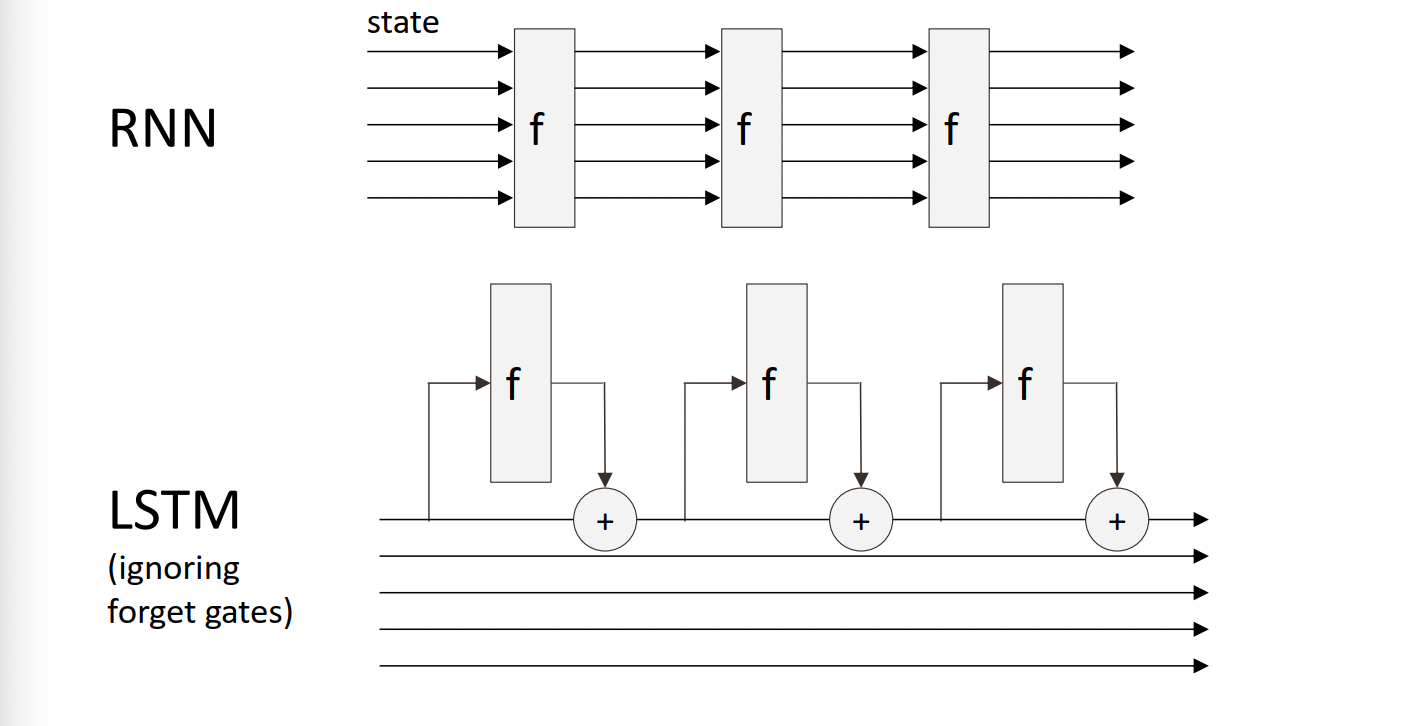
\includegraphics[width=\linewidth]{graphic/rnn-vs-lstm-1}
 		\captionof{figure}{LSTM vs. RNN}
	\end{Figure}
\end{comment}




